\section{D\'{e}marrer un projet en \'{e}quipe}

\begin{frame}
    \begin{center}
    \fontsize{48pt}{7.2}\selectfont
    D\'{e}marrer un projet en \'{e}quipe
    \end{center}
\end{frame}

\subsection{K I S S}
\begin{frame}[fragile]
	\frametitle{K I S S}
	\textbf{Keep It Stupid Simple}, un principe de base valant \`{a} tous les niveaux, du code \`{a} l'organisation de l'\'{e}quipe en passant par l'architecture du projet.
    \\~\\    
	\begin{lstlisting}
private static int sumAbsoluteElements(ArrayList<Integer> list) {
	int sum = 0;

	for (Iterator<Integer> iter = list.iterator(); iter.hasNext();) {
		Integer value = iter.next();
		if (value > 0) {
			sum += value;
		} else {
			sum -= value;
		}
	}

	return sum;
}
	\end{lstlisting}
\end{frame}

\begin{frame}[fragile]
	\frametitle{K I S S}
    
    La simplicit\'{e} est la sophistication supr\^{e}me. (L\'{e}onard De Vinci)
    \\~\\
	\begin{lstlisting}
public int absoluteSum(Collection<Integer> numbers) {
	return numbers.stream().mapToInt(Math::abs).sum();
}
	\end{lstlisting}
\end{frame}


\subsection{C4}

\begin{frame}
	\frametitle{C4 I}
    
    \textbf{C4} est une approche pour concevoir un syst\`{e}me informatique sans compliquer inutilement l'architecture.
    \\~\\
    Pour ce faire, il est n\'{e}cessaire d'\'{e}tablir un ensemble de termes et d'abstractions avec lesquels tous les intervenants du projet pourront se \textbf{comprendre}.
    \\~\\
    C'est une \'{e}tape cruciale, qui permet d'\'{e}viter par la suite d'avoir des incompr\'{e}hension entre les diff\'{e}rents corps de m\'{e}tier (fonctionnels, d\'{e}veloppeurs, int\'{e}grateurs, etc.).
    \\~\\
    Ce sont ces \'{e}l\'{e}ments qui permettront de construire les diagrammes qui seront \`{a} la base du projet.
\end{frame}

\begin{frame}
	\frametitle{C4 II}
    
    Avec cette base, les intervenants peuvent construire le \textbf{diagramme de contexte}.
    \\~\\
    Ce diagramme permet de comprendre les principales fonctionnalit\'{e}s du syst\`{e}me sans afficher comment le syst\`{e}me est organis\'{e}.
    \\~\\
    Le syst\`{e}me est repr\'{e}sent\'{e} par une unique forme (boite noire) qui sera en interaction avec des personnes ou d'autres syst\`{e}mes.
    \\~\\
    Les d\'{e}tails (technologies, protocoles, etc.) n'ont pas d'importance dans ce diagramme, il doit pouvoir \^{e}tre compris par des intervenants non-techniques.
\end{frame}

\begin{frame}
	\frametitle{C4 III}

    \textbf{Exemple de diagramme de contexte}\\
    \centerline{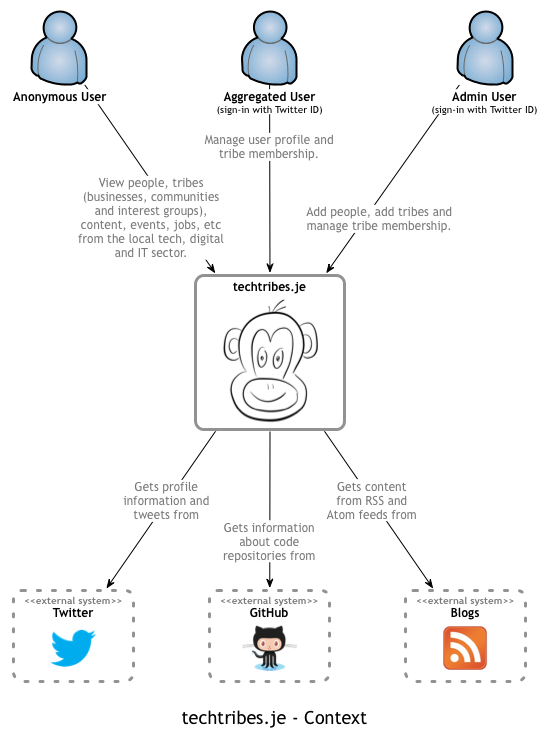
\includegraphics[width=5cm]{img/context_diagram.png}}
\end{frame}

\begin{frame}
	\frametitle{C4 IV}
    
    Une fois les fonctionnalit\'{e}s du syst\`{e}mes acquises, on peut \textit{zoomer} d'un cran avec le \textbf{diagramme de \textit{conteneurs}}.
    \\~\\
    On entend par \textit{conteneur} tout syst\`{e}me qui peut h\'{e}berger du code ou des donn\'{e}es (application, base de donn\'{e}es, broker, etc.).
    \\~\\
    Ce diagramme va refl\'{e}ter l'architecture du syst\`{e}me et permettre de visualiser comment les responsabilit\'{e}s sont r\'{e}parties parmi les diff\'{e}rentes briques logicielles.
    \\~\\
    Ici peuvent \^{e}tre repr\'{e}sent\'{e}s
    \begin{itemize}
    	\item la \textbf{s\'{e}curit\'{e}} : zones r\'{e}seau, flux chiffr\'{e}s, tra\c{c}abilit\'{e}, etc.
        \item la \textbf{scalabilit\'{e}} : load-balancers, (SPOF), etc.
        \item la \textbf{fiabilit\'{e}} : sauvegarde, r\'{e}plication, etc
        \item la \textbf{supervision} : sondes, bases, IHM, etc.
    \end{itemize}
\end{frame}

\begin{frame}
	\frametitle{C4 V}

    \textbf{Exemple de diagramme de conteneurs}\\
    \centerline{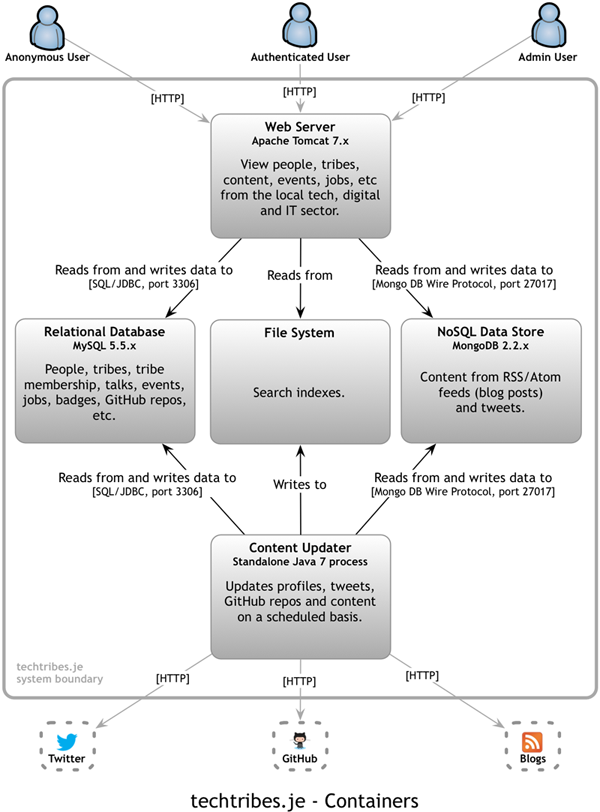
\includegraphics[width=5cm]{img/container_diagram.png}}
\end{frame}

\begin{frame}
	\frametitle{C4 VI}
    
    On peut \`{a} nouveau \textit{zoomer} sur chacun des conteneurs gr\^{a}ce au \textbf{diagramme de composants}.
    \\~\\
    Ce diagramme d\'{e}taille ce dont est compos\'{e} un conteneur, avec un d\'{e}coupage possible par
    \begin{itemize}
    	\item fonctionnalit\'{e} transverse
        \item service m\'{e}tier
        \item workflow
    \end{itemize}
    ~\\
    Un composant a donc une identit\'{e} logique, une \underline{responsabilit\'{e}} et interagit avec d'autres composants.
    \\~\\
    Sont habituellement consign\'{e}s les d\'{e}tails d'impl\'{e}mentation et choix technologiques car ce sch\'{e}ma peut \^{e}tre la documentation la plus d\'{e}taill\'{e}e d'un projet.
\end{frame}

\begin{frame}
	\frametitle{C4 VII}

    \textbf{Exemple de diagramme de composants}\\
    \centerline{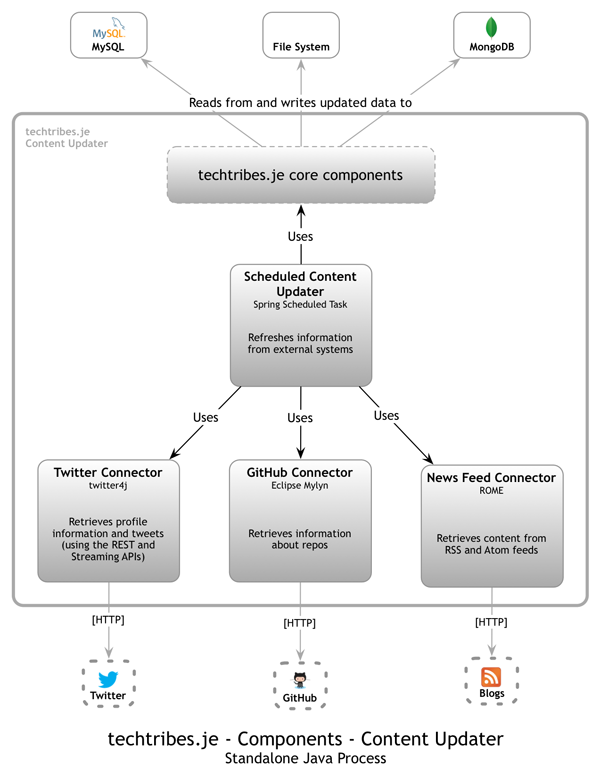
\includegraphics[width=5cm]{img/component_diagram.png}}
\end{frame}

\begin{frame}
	\frametitle{C4 VIII}
    Si n\'{e}cessaire, il est possible de descendre au classique \textbf{diagramme UML de classes}.
    \\~\\
    Ce diagramme est rarement utile si les besoins sont clairs, et les responsabilit\'{e}s bien r\'{e}parties.
    \\~\\
    Cependant, pour mod\'{e}liser un comportement complexe, ce sch\'{e}ma peut mettre en lumi\`{e}re une interaction complexe entre plusieurs objets.
\end{frame}

\begin{frame}
	\frametitle{C4 IX}

    \textbf{Exemple de diagramme de classes}\\
    \centerline{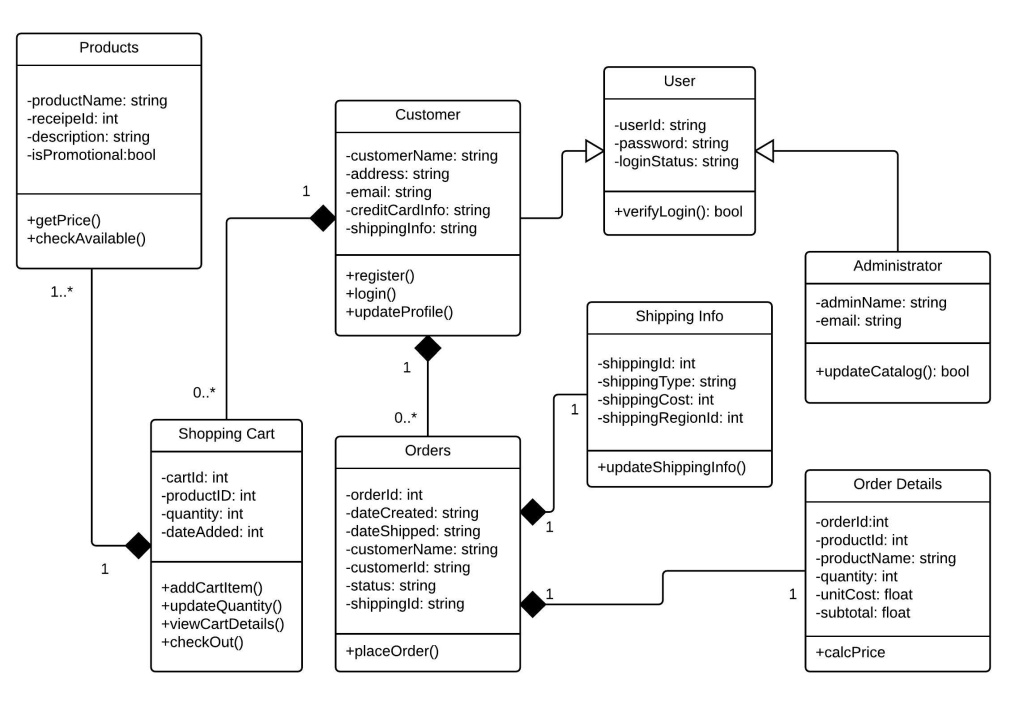
\includegraphics[width=8cm]{img/class_diagram.jpg}}
\end{frame}

\subsection{D\'{e}veloppement pilot\'{e} par les tests (TDD, BDD)}
\begin{frame}
	\frametitle{TDD}
    Le d\'{e}veloppement pilot\'{e} par les tests (\textbf{T}est-\textbf{D}riven \textbf{D}evelopment) consiste \`{a} coder les tests avant l'application.
    \\~\\
    On entend par test principalement les tests unitaires, mais le principe peut \^{e}tre \'{e}tendu \`{a} tous les types, y compris les tests de recette automatis\'{e}s (AT).
    \\~\\
    Afin que le code compile, il est souvent n\'{e}cessaire de coder le squelette du programme, c'est-\`{a}-dire une m\'{e}thode vide.
    \\~\\
    C'est un processus it\'{e}ratif, il n'est pas n\'{e}cessaire de coder tous les tests du premier coup.
    \\~\\
    Tester un code revient \`{a} le brancher dans un autre composant, le composant d\'{e}velopp\'{e} est donc \underline{test\'{e} et facilement utilisable}.
\end{frame}

\begin{frame}
	\frametitle{BDD I}
    Le BDD (\textbf{B}ehavior-\textbf{D}riven \textbf{D}evelopment) est quasiment la m\^{e}me chose que le TDD.
    \\~\\
    La subtilit\'{e} est qu'on ne teste plus une application, mais qu'on d\'{e}finit son comportement.
    \\~\\
    Pour cela le BDD propose d'\'{e}crire en langage naturel, avec une s\'{e}mantique chronologique :
    \begin{itemize}
    	\item Given : les condition initiales
        \item When : \'{e}l\'{e}ment d\'{e}clencheur (unique)
        \item Then : v\'{e}rifications
    \end{itemize}
	~\\
	L'avantage du BDD est de fournir des cahiers de tests lisibles par tous et faciles \`{a} \'{e}crire pour un d\'{e}veloppeur.
\end{frame}

\begin{frame}[fragile]
	\frametitle{BDD II}
    La structure des outils de BDD associant des phrases (patterns) \`{a} du code (m\'{e}thodes), permet naturellement la composition.
    \\~\\
    \begin{lstlisting}[basicstyle=\tiny]
Feature: Owner service

Scenario: Owner list is empty on startup
  Given database is empty
  When an HTTP GET request is made on resource /owner/list
  Then the HTTP response code should be OK
  Then the HTTP response body should be []

Scenario: Owner creation
  Given database is empty
  When an HTTP POST request is made on resource /owner with content
    """
      {
      	"firstName": "Steeve",
      	"lastName": "Jobs"
      }
    """
  Then the HTTP response code should be CREATED
  And an HTTP GET request on resource /owner/list should respond status 200 with body matching
  | Expression                             | Expected result |
  | $[?(@.firstName == 'Steeve')].lastName | Jobs            |
	\end{lstlisting}
\end{frame}

\subsection{Des logs pour tous}
\begin{frame}
	\frametitle{Des logs pour tous I}

    Les logs sont indispensables pour comprendre un dysfonctionnement, elles servent essentiellement de contexte d'ex\'{e}cution.
    \\~\\
    Les logs peuvent \^{e}tre lues par :
    \begin{itemize}
    	\item les d\'{e}veloppeurs
        \item les int\'{e}grateurs
        \item les testeurs (recette)
        \item les administrateurs syst\`{e}me
    \end{itemize}
    ~\\
    C'est pourquoi il est important que les logs soient claires et apportent le maximum d'informations possibles.
    \\~\\
    Pour cela on \'{e}vite les logs visuelles ou de debug.
\end{frame}

\begin{frame}[fragile]
	\frametitle{Des logs pour tous II}

    \begin{lstlisting}[basicstyle=\tiny]
2017-02-04 22:33:12 [main] com.github.lolo.projet.DatabaseService l.74 #################
2017-02-04 22:33:12 [main] com.github.lolo.projet.DatabaseService l.75 START
2017-02-04 22:33:12 [main] com.github.lolo.projet.DatabaseService l.93 STOP in 17ms
2017-02-04 22:33:12 [main] com.github.lolo.projet.DatabaseService l.94 #################
2017-02-04 22:33:12 [main] com.github.lolo.projet.DatabaseService l.124 java.sql.SQLIntegrityConstraintViolationException
	at org.h2.message.DbException.getJdbcSQLException(DbException.java:345)
	at org.h2.message.DbException.get(DbException.java:179)
	at org.h2.message.DbException.get(DbException.java:155)
	at org.h2.command.CommandContainer.update(CommandContainer.java:98)
	at org.h2.command.Command.executeUpdate(Command.java:258)
	at org.h2.jdbc.JdbcPreparedStatement.execute(JdbcPreparedStatement.java:201)
	... 50 more
    \end{lstlisting}
    ~\\
    \'{E}viter les informations inutiles.\\
    Exprimer le \textbf{maximum} en un \textbf{minimum de lignes}.
    \\~\\
    \begin{lstlisting}[basicstyle=\tiny]
2017-02-04 22:33:12.332 INFO  c.g.l.p.UserService.create [Joshua] [Bloch] Save successful
2017-02-04 22:33:12.758 INFO  c.g.l.p.UserService.create [Doug] [Lea] Save successful
2017-02-04 22:33:12.964 ERROR c.g.l.p.UserService.create [James] [Gosling] Save KO: already exists
    \end{lstlisting}
\end{frame}

\begin{frame}[fragile]
	\frametitle{Des logs pour tous III}

    Pour faciliter la cr\'{e}ation de logs, il existe de nombreuses libs.
    \\~\\
    Elles se retrouvent pour la plupart autour de la structure suivante:
     \begin{itemize}
    	\item \textbf{Logger} : recueille les informations \'{e}mises \`{a} divers endroits de l'application
        \item \textbf{Appender} : agr\`{e}ge et sauvegarde les informations (dans un fichier, dans une base, vers un broker, etc.)
    \end{itemize}
    ~\\
    On configure donc habituellement
    \begin{itemize}
    	\item le niveau de verbosit\'{e} (importance) de chaque \textbf{logger}
        \item le format et la destination d'un \textbf{appender}
    \end{itemize}
    
\end{frame}

\begin{frame}[fragile]
	\frametitle{Des logs pour tous IV}

    En utilisant le pattern MDC (\textbf{M}apped \textbf{D}iagnostic \textbf{C}ontext), il est possible de transporter des informations contextuelles : 
    \begin{itemize}
    	\item ID de corr\'{e}lation
        \item param\`{e}tre de service standard
        \item origine d'une requ\^{e}te
        \item ID de run (pour un batch par ex.)
        \item etc.
    \end{itemize}
    ~\\
    Ainsi sans alourdir les appels aux m\'{e}thodes ou aux loggers, les informations sont stock\'{e}es dans le contexte du Thread traitant la requ\^{e}te.
    \\~\\
    Ces informations peuvent ensuite \^{e}tre retrouv\'{e}es directement dans la configuration des appenders.
\end{frame}

\begin{frame}[fragile]
	\frametitle{Des logs pour tous V}

    \begin{lstlisting}[basicstyle=\tiny]
public void onMessage(Message message) {
    MDC.put("ID_MESSAGE", message.getId());
    try {
        service.save(message.getContent());
        LOGGER.info("Save successful");
    } catch(InvalidMessageException e) {
        LOGGER.error("Save KO: " + e.getMessage());
    }
}
    \end{lstlisting}
    ~\\
    \begin{lstlisting}[basicstyle=\tiny]
	<appender name="STDOUT" class="ch.qos.logback.core.ConsoleAppender">
		<encoder>
      		<pattern>%d{yyyy-MM-dd HH:mm:ss} %-5level %logger{36} [%X{ID_MESSAGE}] %msg%n</pattern>
    	</encoder>
	</appender>
    \end{lstlisting}
    ~\\
    \begin{lstlisting}[basicstyle=\tiny]
2017-02-04 22:33:12 INFO  c.g.l.p.MessageListener [78456878] Save successful
2017-02-04 22:33:14 ERROR c.g.l.p.MessageListener [78456879] Save KO: Unable to parse JSON invalid character { at pos 61.
2017-02-04 22:33:12 INFO  c.g.l.p.MessageListener [78456880] Save successful
    \end{lstlisting}
\end{frame}

\begin{frame}[fragile]
	\frametitle{Logs \& Librairies}

    Dans beaucoup de langages, il n'y a pas de standard et les librairies et frameworks ont chacun leur solution de logging.
    \\~\\
    De mani\`{e}re \`{a} centraliser les logs capt\'{e}es par les diff\'{e}rentes librairies de logging, on peut utiliser des \textbf{\textit{bridges}}.
    \\~\\
    Il va s'agir d'intercepter les appels aux diff\'{e}rentes solutions et de les rediriger vers une unique librairie.
    \\~\\
    En Java, SLF4J propose une solution double :
    \begin{itemize}
    	\item une couche d'abstraction permettant de changer d'impl\'{e}mentation sans changer de code
        \item des bridges pour rediriger les logs des autres librairies de log
    \end{itemize}  
\end{frame}

\begin{frame}
	\frametitle{SLF4J}

    \centerline{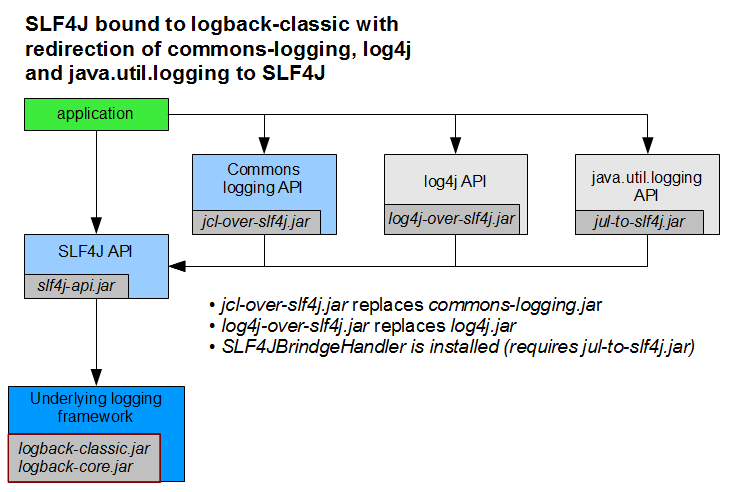
\includegraphics[width=11cm]{img/slf4j.png}}
\end{frame}

\begin{frame}
    \begin{center}
    \fontsize{48pt}{7.2}\selectfont
    D\'{e}mo
    \end{center}
    \begin{center}
    (SLF4J)
    \end{center}
\end{frame}
